 \documentclass{article}
\usepackage[utf8]{inputenc}
\usepackage[a4paper, total={7in, 10in}]{geometry}
\usepackage{braket}
\usepackage{xcolor}
\usepackage{amsmath}
\usepackage{amssymb}
\usepackage{amsfonts}
\usepackage{graphicx}
\usepackage{svg}
\usepackage{float}
\usepackage{tikz}
\usepackage[ruled,vlined]{algorithm2e}
\usepackage{multicol}
\usepackage[backend=biber,style=alphabetic,sorting=ynt]{biblatex}
\usepackage{xcolor}
%\addbibresource{sample.bib} %Import the bibliography file

\newcommand{\commentt}[1]{\textcolor{blue}{ \textbf{[COMMENT]} #1}}
\newcommand{\ctt}[1]{\commentt{#1}}
\newcommand{\prb}[1]{ \mathbf{Pr} \left[ {#1} \right]}
\newcommand{\onotation}[1]{\(\mathcal{O} \left( {#1}  \right) \)}
\newcommand{\ona}[1]{\onotation{#1}}
\newcommand{\PSI}{{\ket{\psi}}}
\newcommand{\LESn}{\ket{\psi_n}}
\newcommand{\LESa}{\ket{\phi_n}}
\newcommand{\LESs}{\frac{1}{\sqrt{n}}\sum_{i}{\ket{\left(0^{i}10^{n-i}\right)^{n}}}}
\newcommand{\Hn}{\mathcal{H}_{n}}
\newcommand{\Ep}{\frac{1}{\sqrt{2^n}}\sum^{2^n}_{x}{ \ket{xx}}}
\newcommand{\HON}{\ket{\psi_{\text{honest}}}}
\newcommand{\Lemma}{\paragraph{Lemma.}}


\setlength{\columnsep}{0.6cm}

\newcommand{\Gz}{ G_{z}^{\delta} } 

\begin{document}

\title{Quantum LTC With Positive Rate}
\author{David Ponarovsky}
\maketitle
%\begin{multicols*}{2}
\newcommand{ \Hw }{ \delta\Delta -\Delta^{\frac{1}{2}-\varepsilon}/\delta  }
	\newcommand{ \Nw }{ \Delta^{\frac{3}{2}-\varepsilon}} 
	  \newcommand{ \Gu } { \Gamma^{\cup} }
	  \newcommand{ \Guq } { \Gamma^{\cup, \square} }

    	\newcommand{ \Gsa } {\Gamma_{\square_{1}} }
	\newcommand{ \Gsb } {\Gamma_{\square_{2}} }
        \newcommand{ \Aa } { C_{A_{1}}}  
	\newcommand{ \Ab } { C_{A_{2}}}
	\newcommand{ \Ac } { C_{A_{3}}}
	\newcommand{ \Aab } { \Aa \otimes \Ab } 
	\newcommand{ \Aac } { \Aa \otimes \Ac }
	\newcommand{ \Aabc } { \Aa \otimes \Ab \otimes \Ac }
	\newcommand{ \Aabp } { \Aa^{\perp} \otimes \Ab^{\perp} } 
	\newcommand{ \Aacp } { \Aa^{\perp} \otimes \Ac^{\perp} }
	\newcommand{ \Aabcp } { \Aa^{\perp} \otimes \Ab^{\perp} \otimes \Ac^{\perp} }
	\newcommand{ \Aabpp } { \left( \Aabp \right)^\perp } 
	\newcommand{ \Aacpp } { \left( \Aacp \right)^\perp }
	\newcommand{ \Aabcpp } { \left( \Aabcp \right)^\perp }
	\newcommand{ \YY } {  y_{1}y_{2}^{\top} }
	\newcommand{ \ZZ } {  z_{1}z_{2}^{\top} } 
	\newcommand{ \TT } { \tilde{\tau} } 


  \paragraph{preamble.} preamble.  
  \begin{figure}[H]
            %\label{fig:square}
            \begin{center}
            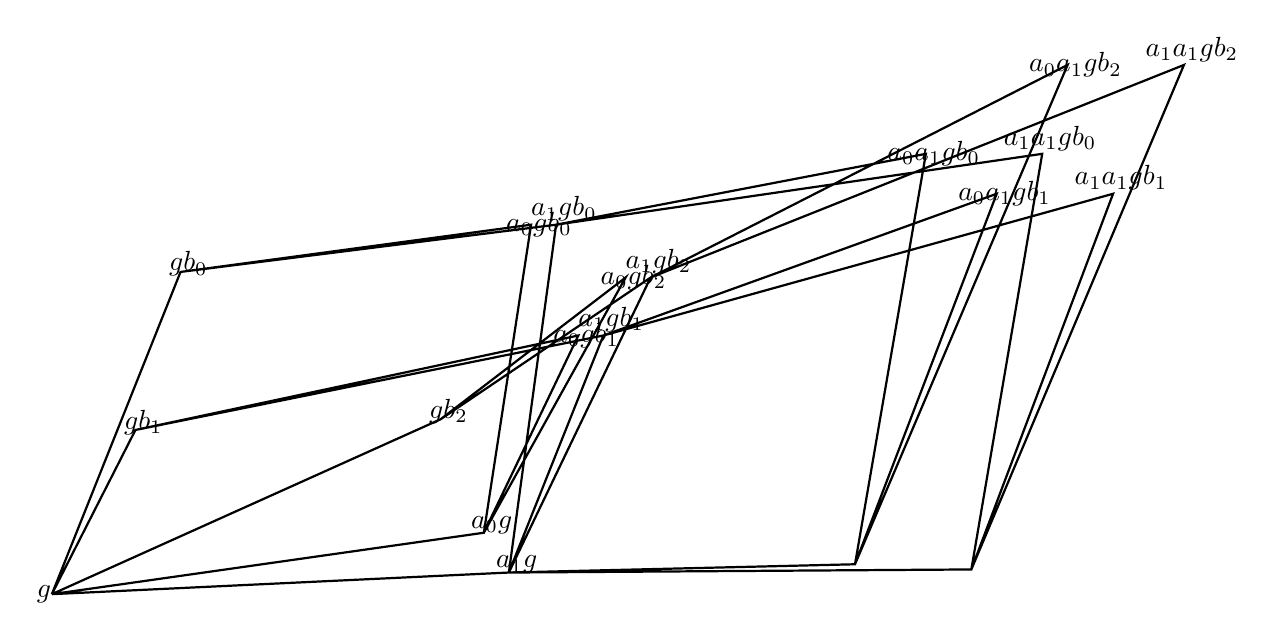
\begin{tikzpicture}
            \draw[thick](0,0)(0, 0) -- (1.633866230646458,4.092162648693855) -- (6.086031133411885,4.692162648693855) -- (5.486031133411886,0.7799969271715819) -- (0, 0)
(0, 0) -- (1.0614259332640763,2.08506700209454) -- (6.686031133411886,3.2850670020945403) -- (5.486031133411886,0.7799969271715819) -- (0, 0)
(0, 0) -- (4.936703418070688,2.221067298010628) -- (7.2860311334118855,4.021067298010628) -- (5.486031133411886,0.7799969271715819) -- (0, 0)
(0, 0) -- (1.633866230646458,4.092162648693855) -- (6.403634681274485,4.692162648693855) -- (5.8036346812744855,0.2747075203019409) -- (0, 0)
(0, 0) -- (1.0614259332640763,2.08506700209454) -- (7.003634681274486,3.2850670020945403) -- (5.8036346812744855,0.2747075203019409) -- (0, 0)
(0, 0) -- (4.936703418070688,2.221067298010628) -- (7.603634681274485,4.021067298010628) -- (5.8036346812744855,0.2747075203019409) -- (0, 0)
(5.8036346812744855, 0.2747075203019409) -- (6.403634681274485,4.692162648693855) -- (11.099616075160457,5.592162648693855) -- (10.199616075160456,0.37964219238192215) -- (5.8036346812744855, 0.2747075203019409)
(5.8036346812744855, 0.2747075203019409) -- (7.003634681274486,3.2850670020945403) -- (11.999616075160457,5.08506700209454) -- (10.199616075160456,0.37964219238192215) -- (5.8036346812744855, 0.2747075203019409)
(5.8036346812744855, 0.2747075203019409) -- (7.603634681274485,4.021067298010628) -- (12.899616075160456,6.721067298010628) -- (10.199616075160456,0.37964219238192215) -- (5.8036346812744855, 0.2747075203019409)
(5.8036346812744855, 0.2747075203019409) -- (6.403634681274485,4.692162648693855) -- (12.577226810308881,5.592162648693855) -- (11.67722681030888,0.3137470971501795) -- (5.8036346812744855, 0.2747075203019409)
(5.8036346812744855, 0.2747075203019409) -- (7.003634681274486,3.2850670020945403) -- (13.477226810308881,5.08506700209454) -- (11.67722681030888,0.3137470971501795) -- (5.8036346812744855, 0.2747075203019409)
(5.8036346812744855, 0.2747075203019409) -- (7.603634681274485,4.021067298010628) -- (14.37722681030888,6.721067298010628) -- (11.67722681030888,0.3137470971501795) -- (5.8036346812744855, 0.2747075203019409)
;
\node at (6.186031133411885,4.692162648693855) {$ a_{ 0  } gb_{ 0 } $};
\node at (6.7860311334118855,3.2850670020945403) {$ a_{ 0  } gb_{ 1 } $};
\node at (7.386031133411885,4.021067298010628) {$ a_{ 0  } gb_{ 2 } $};
\node at (6.503634681274485,4.892162648693855) {$ a_{ 1  } gb_{ 0 } $};
\node at (7.103634681274485,3.4850670020945405) {$ a_{ 1  } gb_{ 1 } $};
\node at (7.703634681274485,4.221067298010628) {$ a_{ 1  } gb_{ 2 } $};
\node at (11.199616075160456,5.592162648693855) {$ a_{ 0  } a_{ 1 }gb_{ 0 } $};
\node at (12.099616075160457,5.08506700209454) {$ a_{ 0  } a_{ 1 }gb_{ 1 } $};
\node at (12.999616075160455,6.721067298010628) {$ a_{ 0  } a_{ 1 }gb_{ 2 } $};
\node at (12.67722681030888,5.792162648693855) {$ a_{ 1  } a_{ 1 }gb_{ 0 } $};
\node at (13.577226810308881,5.28506700209454) {$ a_{ 1  } a_{ 1 }gb_{ 1 } $};
\node at (14.47722681030888,6.9210672980106285) {$ a_{ 1  } a_{ 1 }gb_{ 2 } $};
\node at (-0.1,0) {$ g $};
\node at (5.586031133411885,0.8799969271715818) {$ a_{ 0 }g $};
\node at (5.903634681274485,0.3747075203019409) {$ a_{ 1 }g $};
\node at (1.733866230646458,4.192162648693855) {$ gb_{ 0 } $};
\node at (1.1614259332640764,2.18506700209454) {$ gb_{ 1 } $};
\node at (5.0367034180706876,2.321067298010628) {$ gb_{ 2 } $};

            \end{tikzpicture}
            \end{center}
            \caption{Square of the complex, with edges $(g,ag), (agb, gb) \in E_A,
            (g,gb), (agb, ag) \in E_B.$ \label{fig:square}
            }
            \end{figure}
 \begin{figure}[H]
            %\label{fig:square}
            \begin{center}
            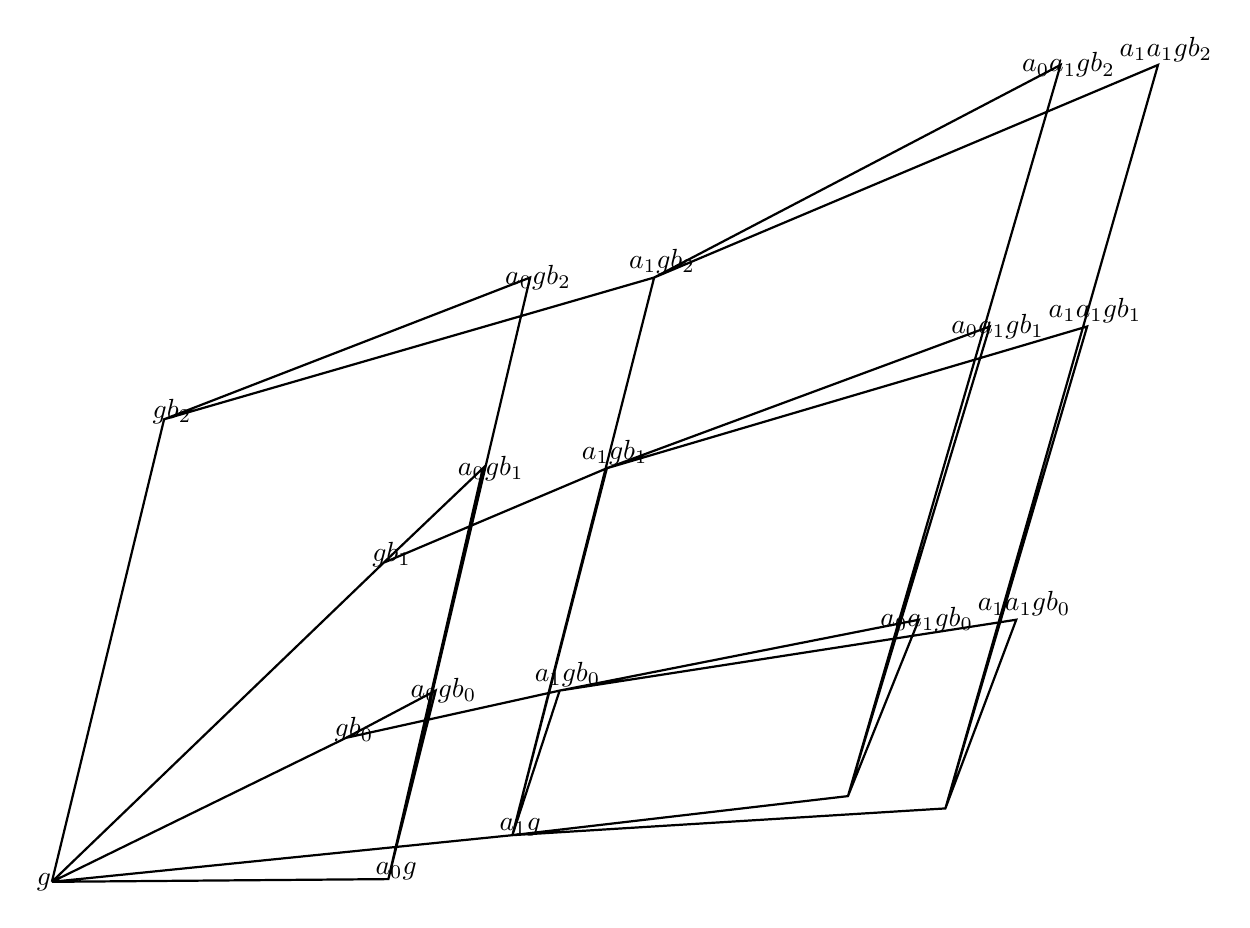
\begin{tikzpicture}
            \draw[thick](0,0)(0, 0) -- (3.7365912467150144,1.8286842712378273) -- (4.873428620253003,2.4286842712378274) -- (4.273428620253004,0.034482968256904334) -- (0, 0)
(0, 0) -- (4.213589110971676,4.0525744678612865) -- (5.473428620253004,5.252574467861287) -- (4.273428620253004,0.034482968256904334) -- (0, 0)
(0, 0) -- (1.4255305896063575,5.874361851684012) -- (6.0734286202530035,7.6743618516840115) -- (4.273428620253004,0.034482968256904334) -- (0, 0)
(0, 0) -- (3.7365912467150144,1.8286842712378273) -- (6.448748349061763,2.4286842712378274) -- (5.848748349061763,0.5924744220088068) -- (0, 0)
(0, 0) -- (4.213589110971676,4.0525744678612865) -- (7.048748349061763,5.252574467861287) -- (5.848748349061763,0.5924744220088068) -- (0, 0)
(0, 0) -- (1.4255305896063575,5.874361851684012) -- (7.648748349061763,7.6743618516840115) -- (5.848748349061763,0.5924744220088068) -- (0, 0)
(5.848748349061763, 0.5924744220088068) -- (6.448748349061763,2.4286842712378274) -- (11.010439011740969,3.3286842712378273) -- (10.110439011740969,1.0885955245997985) -- (5.848748349061763, 0.5924744220088068)
(5.848748349061763, 0.5924744220088068) -- (7.048748349061763,5.252574467861287) -- (11.91043901174097,7.0525744678612865) -- (10.110439011740969,1.0885955245997985) -- (5.848748349061763, 0.5924744220088068)
(5.848748349061763, 0.5924744220088068) -- (7.648748349061763,7.6743618516840115) -- (12.810439011740968,10.37436185168401) -- (10.110439011740969,1.0885955245997985) -- (5.848748349061763, 0.5924744220088068)
(5.848748349061763, 0.5924744220088068) -- (6.448748349061763,2.4286842712378274) -- (12.247659505463124,3.3286842712378273) -- (11.347659505463124,0.9322255623854454) -- (5.848748349061763, 0.5924744220088068)
(5.848748349061763, 0.5924744220088068) -- (7.048748349061763,5.252574467861287) -- (13.147659505463125,7.0525744678612865) -- (11.347659505463124,0.9322255623854454) -- (5.848748349061763, 0.5924744220088068)
(5.848748349061763, 0.5924744220088068) -- (7.648748349061763,7.6743618516840115) -- (14.047659505463123,10.37436185168401) -- (11.347659505463124,0.9322255623854454) -- (5.848748349061763, 0.5924744220088068)
;
\node at (4.973428620253003,2.4286842712378274) {$ a_{ 0  } gb_{ 0 } $};
\node at (5.5734286202530035,5.252574467861287) {$ a_{ 0  } gb_{ 1 } $};
\node at (6.173428620253003,7.6743618516840115) {$ a_{ 0  } gb_{ 2 } $};
\node at (6.548748349061762,2.6286842712378276) {$ a_{ 1  } gb_{ 0 } $};
\node at (7.148748349061763,5.452574467861287) {$ a_{ 1  } gb_{ 1 } $};
\node at (7.748748349061763,7.874361851684012) {$ a_{ 1  } gb_{ 2 } $};
\node at (11.110439011740969,3.3286842712378273) {$ a_{ 0  } a_{ 1 }gb_{ 0 } $};
\node at (12.010439011740969,7.0525744678612865) {$ a_{ 0  } a_{ 1 }gb_{ 1 } $};
\node at (12.910439011740968,10.37436185168401) {$ a_{ 0  } a_{ 1 }gb_{ 2 } $};
\node at (12.347659505463124,3.5286842712378275) {$ a_{ 1  } a_{ 1 }gb_{ 0 } $};
\node at (13.247659505463124,7.252574467861287) {$ a_{ 1  } a_{ 1 }gb_{ 1 } $};
\node at (14.147659505463123,10.57436185168401) {$ a_{ 1  } a_{ 1 }gb_{ 2 } $};
\node at (-0.1,0) {$ g $};
\node at (4.373428620253003,0.13448296825690434) {$ a_{ 0 }g $};
\node at (5.948748349061763,0.6924744220088068) {$ a_{ 1 }g $};
\node at (3.8365912467150145,1.9286842712378274) {$ gb_{ 0 } $};
\node at (4.313589110971676,4.152574467861286) {$ gb_{ 1 } $};
\node at (1.5255305896063576,5.974361851684011) {$ gb_{ 2 } $};

            \end{tikzpicture}
            \end{center}
            \caption{Square of the complex, with edges $(g,ag), (agb, gb) \in E_A,
            (g,gb), (agb, ag) \in E_B.$ \label{fig:square}
            }
            \end{figure}
 \begin{figure}[H]
            %\label{fig:square}
            \begin{center}
            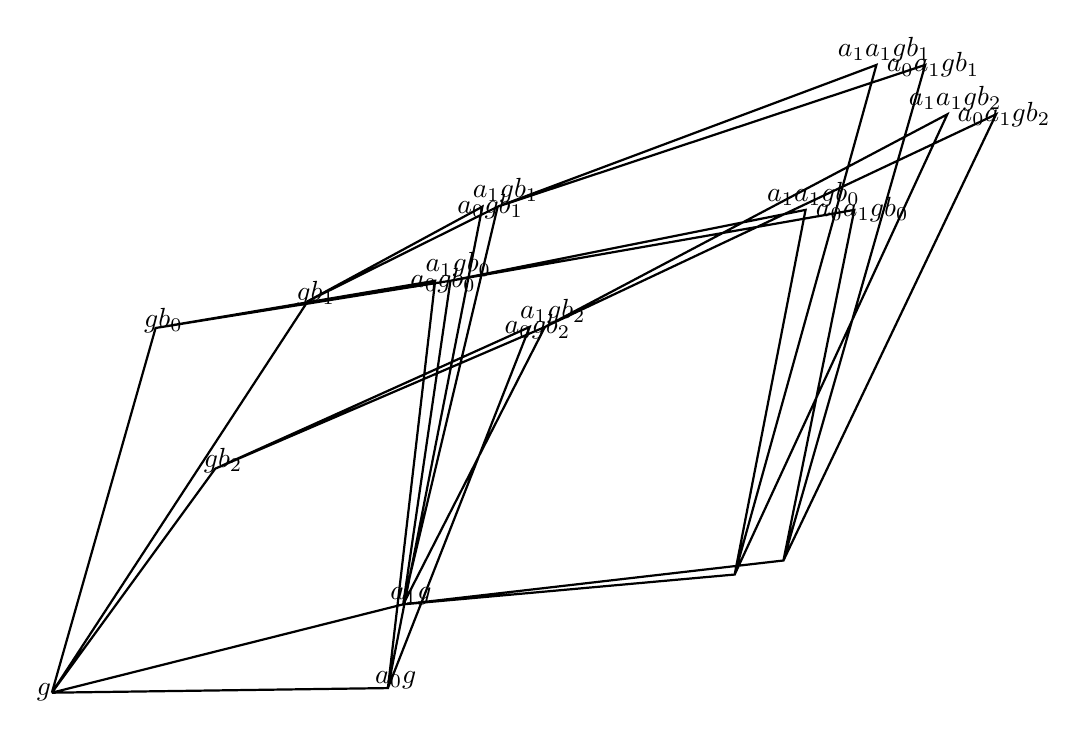
\begin{tikzpicture}
            \draw[thick](0,0)(0, 0) -- (1.3174769499766248,4.631572094750734) -- (4.867578136937819,5.231572094750733) -- (4.26757813693782,0.05856396485048081) -- (0, 0)
(0, 0) -- (3.2508800801243094,4.9723875231800925) -- (5.46757813693782,6.172387523180093) -- (4.26757813693782,0.05856396485048081) -- (0, 0)
(0, 0) -- (2.0747380453065105,2.8449983648652344) -- (6.067578136937819,4.644998364865234) -- (4.26757813693782,0.05856396485048081) -- (0, 0)
(0, 0) -- (1.3174769499766248,4.631572094750734) -- (5.061856351436948,5.231572094750733) -- (4.461856351436948,1.1220783288673066) -- (0, 0)
(0, 0) -- (3.2508800801243094,4.9723875231800925) -- (5.661856351436948,6.172387523180093) -- (4.461856351436948,1.1220783288673066) -- (0, 0)
(0, 0) -- (2.0747380453065105,2.8449983648652344) -- (6.261856351436948,4.644998364865234) -- (4.461856351436948,1.1220783288673066) -- (0, 0)
(4.461856351436948, 1.1220783288673066) -- (5.061856351436948,5.231572094750733) -- (10.190996266235096,6.131572094750734) -- (9.290996266235096,1.678834766279731) -- (4.461856351436948, 1.1220783288673066)
(4.461856351436948, 1.1220783288673066) -- (5.661856351436948,6.172387523180093) -- (11.090996266235097,7.9723875231800925) -- (9.290996266235096,1.678834766279731) -- (4.461856351436948, 1.1220783288673066)
(4.461856351436948, 1.1220783288673066) -- (6.261856351436948,4.644998364865234) -- (11.990996266235097,7.344998364865234) -- (9.290996266235096,1.678834766279731) -- (4.461856351436948, 1.1220783288673066)
(4.461856351436948, 1.1220783288673066) -- (5.061856351436948,5.231572094750733) -- (9.571588709408456,6.131572094750734) -- (8.671588709408455,1.500621224306397) -- (4.461856351436948, 1.1220783288673066)
(4.461856351436948, 1.1220783288673066) -- (5.661856351436948,6.172387523180093) -- (10.471588709408456,7.9723875231800925) -- (8.671588709408455,1.500621224306397) -- (4.461856351436948, 1.1220783288673066)
(4.461856351436948, 1.1220783288673066) -- (6.261856351436948,4.644998364865234) -- (11.371588709408456,7.344998364865234) -- (8.671588709408455,1.500621224306397) -- (4.461856351436948, 1.1220783288673066)
;
\node at (4.967578136937819,5.231572094750733) {$ a_{ 0  } gb_{ 0 } $};
\node at (5.567578136937819,6.172387523180093) {$ a_{ 0  } gb_{ 1 } $};
\node at (6.167578136937819,4.644998364865234) {$ a_{ 0  } gb_{ 2 } $};
\node at (5.161856351436947,5.4315720947507335) {$ a_{ 1  } gb_{ 0 } $};
\node at (5.761856351436948,6.372387523180093) {$ a_{ 1  } gb_{ 1 } $};
\node at (6.3618563514369475,4.844998364865234) {$ a_{ 1  } gb_{ 2 } $};
\node at (10.290996266235096,6.131572094750734) {$ a_{ 0  } a_{ 1 }gb_{ 0 } $};
\node at (11.190996266235096,7.9723875231800925) {$ a_{ 0  } a_{ 1 }gb_{ 1 } $};
\node at (12.090996266235097,7.344998364865234) {$ a_{ 0  } a_{ 1 }gb_{ 2 } $};
\node at (9.671588709408455,6.331572094750734) {$ a_{ 1  } a_{ 1 }gb_{ 0 } $};
\node at (10.571588709408456,8.172387523180092) {$ a_{ 1  } a_{ 1 }gb_{ 1 } $};
\node at (11.471588709408456,7.544998364865235) {$ a_{ 1  } a_{ 1 }gb_{ 2 } $};
\node at (-0.1,0) {$ g $};
\node at (4.367578136937819,0.1585639648504808) {$ a_{ 0 }g $};
\node at (4.561856351436948,1.2220783288673067) {$ a_{ 1 }g $};
\node at (1.4174769499766249,4.731572094750733) {$ gb_{ 0 } $};
\node at (3.3508800801243095,5.072387523180092) {$ gb_{ 1 } $};
\node at (2.1747380453065106,2.9449983648652345) {$ gb_{ 2 } $};

            \end{tikzpicture}
            \end{center}
            \caption{Square of the complex, with edges $(g,ag), (agb, gb) \in E_A,
            (g,gb), (agb, ag) \in E_B.$ \label{fig:square}
            }
            \end{figure}
 \begin{figure}[H]
            %\label{fig:square}
            \begin{center}
            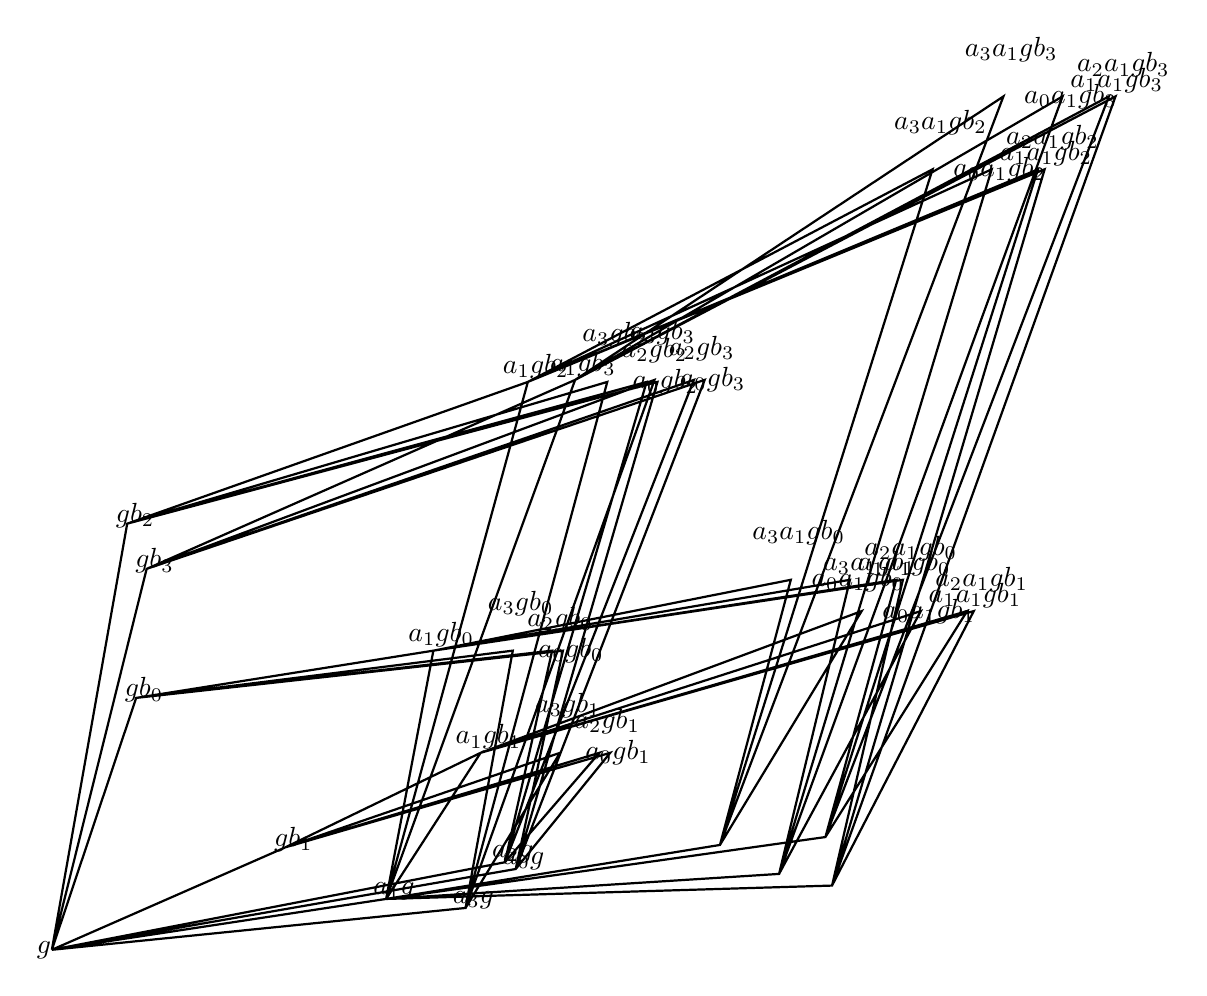
\begin{tikzpicture}
            \draw[thick](0,0)(0, 0) -- (1.0704730681850898,3.198886242749492) -- (6.490688607395355,3.798886242749492) -- (5.890688607395355,1.0258891700109) -- (0, 0)
(0, 0) -- (2.966145890509267,1.3014546795710564) -- (7.0906886073953554,2.501454679571056) -- (5.890688607395355,1.0258891700109) -- (0, 0)
(0, 0) -- (0.9568344480347996,5.4117350170490095) -- (7.690688607395355,7.211735017049009) -- (5.890688607395355,1.0258891700109) -- (0, 0)
(0, 0) -- (1.2036000690479458,4.837516124070415) -- (8.290688607395355,7.237516124070416) -- (5.890688607395355,1.0258891700109) -- (0, 0)
(0, 0) -- (1.0704730681850898,3.198886242749492) -- (4.845084634523936,3.798886242749492) -- (4.245084634523936,0.6456649023787898) -- (0, 0)
(0, 0) -- (2.966145890509267,1.3014546795710564) -- (5.445084634523936,2.501454679571056) -- (4.245084634523936,0.6456649023787898) -- (0, 0)
(0, 0) -- (0.9568344480347996,5.4117350170490095) -- (6.045084634523936,7.211735017049009) -- (4.245084634523936,0.6456649023787898) -- (0, 0)
(0, 0) -- (1.2036000690479458,4.837516124070415) -- (6.645084634523936,7.237516124070416) -- (4.245084634523936,0.6456649023787898) -- (0, 0)
(0, 0) -- (1.0704730681850898,3.198886242749492) -- (6.3534927098997915,3.798886242749492) -- (5.753492709899792,1.111607466200753) -- (0, 0)
(0, 0) -- (2.966145890509267,1.3014546795710564) -- (6.953492709899792,2.501454679571056) -- (5.753492709899792,1.111607466200753) -- (0, 0)
(0, 0) -- (0.9568344480347996,5.4117350170490095) -- (7.553492709899792,7.211735017049009) -- (5.753492709899792,1.111607466200753) -- (0, 0)
(0, 0) -- (1.2036000690479458,4.837516124070415) -- (8.153492709899792,7.237516124070416) -- (5.753492709899792,1.111607466200753) -- (0, 0)
(0, 0) -- (1.0704730681850898,3.198886242749492) -- (5.853540900605728,3.798886242749492) -- (5.253540900605729,0.5312014257444966) -- (0, 0)
(0, 0) -- (2.966145890509267,1.3014546795710564) -- (6.453540900605729,2.501454679571056) -- (5.253540900605729,0.5312014257444966) -- (0, 0)
(0, 0) -- (0.9568344480347996,5.4117350170490095) -- (7.053540900605729,7.211735017049009) -- (5.253540900605729,0.5312014257444966) -- (0, 0)
(0, 0) -- (1.2036000690479458,4.837516124070415) -- (7.653540900605728,7.237516124070416) -- (5.253540900605729,0.5312014257444966) -- (0, 0)
(4.245084634523936, 0.6456649023787898) -- (4.845084634523936,3.798886242749492) -- (10.135485880737617,4.698886242749492) -- (9.235485880737617,0.9636366909073578) -- (4.245084634523936, 0.6456649023787898)
(4.245084634523936, 0.6456649023787898) -- (5.445084634523936,2.501454679571056) -- (11.035485880737617,4.301454679571056) -- (9.235485880737617,0.9636366909073578) -- (4.245084634523936, 0.6456649023787898)
(4.245084634523936, 0.6456649023787898) -- (6.045084634523936,7.211735017049009) -- (11.935485880737616,9.91173501704901) -- (9.235485880737617,0.9636366909073578) -- (4.245084634523936, 0.6456649023787898)
(4.245084634523936, 0.6456649023787898) -- (6.645084634523936,7.237516124070416) -- (12.835485880737616,10.837516124070415) -- (9.235485880737617,0.9636366909073578) -- (4.245084634523936, 0.6456649023787898)
(4.245084634523936, 0.6456649023787898) -- (4.845084634523936,3.798886242749492) -- (10.723779432327595,4.698886242749492) -- (9.823779432327594,1.4317916349882864) -- (4.245084634523936, 0.6456649023787898)
(4.245084634523936, 0.6456649023787898) -- (5.445084634523936,2.501454679571056) -- (11.623779432327595,4.301454679571056) -- (9.823779432327594,1.4317916349882864) -- (4.245084634523936, 0.6456649023787898)
(4.245084634523936, 0.6456649023787898) -- (6.045084634523936,7.211735017049009) -- (12.523779432327593,9.91173501704901) -- (9.823779432327594,1.4317916349882864) -- (4.245084634523936, 0.6456649023787898)
(4.245084634523936, 0.6456649023787898) -- (6.645084634523936,7.237516124070416) -- (13.423779432327594,10.837516124070415) -- (9.823779432327594,1.4317916349882864) -- (4.245084634523936, 0.6456649023787898)
(4.245084634523936, 0.6456649023787898) -- (4.845084634523936,3.798886242749492) -- (10.808091797946306,4.698886242749492) -- (9.908091797946305,0.8154771238600342) -- (4.245084634523936, 0.6456649023787898)
(4.245084634523936, 0.6456649023787898) -- (5.445084634523936,2.501454679571056) -- (11.708091797946306,4.301454679571056) -- (9.908091797946305,0.8154771238600342) -- (4.245084634523936, 0.6456649023787898)
(4.245084634523936, 0.6456649023787898) -- (6.045084634523936,7.211735017049009) -- (12.608091797946305,9.91173501704901) -- (9.908091797946305,0.8154771238600342) -- (4.245084634523936, 0.6456649023787898)
(4.245084634523936, 0.6456649023787898) -- (6.645084634523936,7.237516124070416) -- (13.508091797946305,10.837516124070415) -- (9.908091797946305,0.8154771238600342) -- (4.245084634523936, 0.6456649023787898)
(4.245084634523936, 0.6456649023787898) -- (4.845084634523936,3.798886242749492) -- (9.384530725120078,4.698886242749492) -- (8.484530725120077,1.3313667657506958) -- (4.245084634523936, 0.6456649023787898)
(4.245084634523936, 0.6456649023787898) -- (5.445084634523936,2.501454679571056) -- (10.284530725120078,4.301454679571056) -- (8.484530725120077,1.3313667657506958) -- (4.245084634523936, 0.6456649023787898)
(4.245084634523936, 0.6456649023787898) -- (6.045084634523936,7.211735017049009) -- (11.184530725120077,9.91173501704901) -- (8.484530725120077,1.3313667657506958) -- (4.245084634523936, 0.6456649023787898)
(4.245084634523936, 0.6456649023787898) -- (6.645084634523936,7.237516124070416) -- (12.084530725120077,10.837516124070415) -- (8.484530725120077,1.3313667657506958) -- (4.245084634523936, 0.6456649023787898)
;
\node at (6.590688607395355,3.798886242749492) {$ a_{ 0  } gb_{ 0 } $};
\node at (7.190688607395355,2.501454679571056) {$ a_{ 0  } gb_{ 1 } $};
\node at (7.790688607395355,7.211735017049009) {$ a_{ 0  } gb_{ 2 } $};
\node at (8.390688607395354,7.237516124070416) {$ a_{ 0  } gb_{ 3 } $};
\node at (4.945084634523935,3.9988862427494922) {$ a_{ 1  } gb_{ 0 } $};
\node at (5.545084634523936,2.7014546795710563) {$ a_{ 1  } gb_{ 1 } $};
\node at (6.145084634523935,7.4117350170490095) {$ a_{ 1  } gb_{ 2 } $};
\node at (6.745084634523936,7.437516124070416) {$ a_{ 1  } gb_{ 3 } $};
\node at (6.453492709899791,4.198886242749492) {$ a_{ 2  } gb_{ 0 } $};
\node at (7.053492709899792,2.901454679571056) {$ a_{ 2  } gb_{ 1 } $};
\node at (7.653492709899791,7.61173501704901) {$ a_{ 2  } gb_{ 2 } $};
\node at (8.253492709899792,7.637516124070416) {$ a_{ 2  } gb_{ 3 } $};
\node at (5.953540900605728,4.398886242749493) {$ a_{ 3  } gb_{ 0 } $};
\node at (6.553540900605729,3.1014546795710562) {$ a_{ 3  } gb_{ 1 } $};
\node at (7.153540900605728,7.81173501704901) {$ a_{ 3  } gb_{ 2 } $};
\node at (7.753540900605728,7.837516124070415) {$ a_{ 3  } gb_{ 3 } $};
\node at (10.235485880737617,4.698886242749492) {$ a_{ 0  } a_{ 1 }gb_{ 0 } $};
\node at (11.135485880737617,4.301454679571056) {$ a_{ 0  } a_{ 1 }gb_{ 1 } $};
\node at (12.035485880737616,9.91173501704901) {$ a_{ 0  } a_{ 1 }gb_{ 2 } $};
\node at (12.935485880737616,10.837516124070415) {$ a_{ 0  } a_{ 1 }gb_{ 3 } $};
\node at (10.823779432327594,4.898886242749493) {$ a_{ 1  } a_{ 1 }gb_{ 0 } $};
\node at (11.723779432327595,4.501454679571056) {$ a_{ 1  } a_{ 1 }gb_{ 1 } $};
\node at (12.623779432327593,10.111735017049009) {$ a_{ 1  } a_{ 1 }gb_{ 2 } $};
\node at (13.523779432327593,11.037516124070414) {$ a_{ 1  } a_{ 1 }gb_{ 3 } $};
\node at (10.908091797946305,5.098886242749493) {$ a_{ 2  } a_{ 1 }gb_{ 0 } $};
\node at (11.808091797946306,4.701454679571056) {$ a_{ 2  } a_{ 1 }gb_{ 1 } $};
\node at (12.708091797946304,10.31173501704901) {$ a_{ 2  } a_{ 1 }gb_{ 2 } $};
\node at (13.608091797946305,11.237516124070416) {$ a_{ 2  } a_{ 1 }gb_{ 3 } $};
\node at (9.484530725120077,5.298886242749493) {$ a_{ 3  } a_{ 1 }gb_{ 0 } $};
\node at (10.384530725120078,4.9014546795710565) {$ a_{ 3  } a_{ 1 }gb_{ 1 } $};
\node at (11.284530725120076,10.51173501704901) {$ a_{ 3  } a_{ 1 }gb_{ 2 } $};
\node at (12.184530725120077,11.437516124070415) {$ a_{ 3  } a_{ 1 }gb_{ 3 } $};
\node at (-0.1,0) {$ g $};
\node at (5.990688607395355,1.1258891700109002) {$ a_{ 0 }g $};
\node at (4.345084634523936,0.7456649023787898) {$ a_{ 1 }g $};
\node at (5.8534927098997915,1.211607466200753) {$ a_{ 2 }g $};
\node at (5.353540900605728,0.6312014257444966) {$ a_{ 3 }g $};
\node at (1.17047306818509,3.298886242749492) {$ gb_{ 0 } $};
\node at (3.066145890509267,1.4014546795710565) {$ gb_{ 1 } $};
\node at (1.0568344480347995,5.511735017049009) {$ gb_{ 2 } $};
\node at (1.303600069047946,4.937516124070415) {$ gb_{ 3 } $};

            \end{tikzpicture}
            \end{center}
            \caption{Square of the complex, with edges $(g,ag), (agb, gb) \in E_A,
            (g,gb), (agb, ag) \in E_B.$ \label{fig:square}
            }
            \end{figure}
 
%\end{multicols*}
  % \printbibliography 
\end{document}

 